\section{ECOSTRESS Thermal Verification and 25-Year Landsat Panel}
\label{sec:thermal_25yr}

Optical phenology alone cannot directly observe cold-air pooling. Merging NASA \texttt{ECOSTRESS} Collection~2 (2020--2024, 144 granules) with Bayesian cloud-masked Collection~3 (2018--2019 and 2025--2026) yields 157 unique in-swath nighttime passes over Sewanee, of which 60 pass standard cloud and QA flags. Auditing those 60 scenes against co-located ERA5-Land 2~m air temperature uncovered 8 unflagged \texttt{ECOv002} anomalies ($|\text{LST}-\text{ERA5}_{t2m}| > 10^\circ$C; 0/14 clean \texttt{v003} scenes affected): seven cloud-contaminated passes reading $11$--$22^\circ$C colder than surface air temperature (including all three scenes with $u_{10} \ge 3.0$~m/s) and one calibration-corrupted pre-dawn pass reading $+46$--$48^\circ$C. Applying a physical $|\text{LST}-\text{ERA5}_{t2m}| \le 10^\circ$C filter retains $n=52$ clean nights ($38$ \texttt{v002}, $14$ \texttt{v003}; $51$ with matched ERA5 wind, as one November 2026 \texttt{v003} scene precedes ERA5 publication; \cref{fig:ecostress_thermal}).

\begin{figure}[t]
\centering
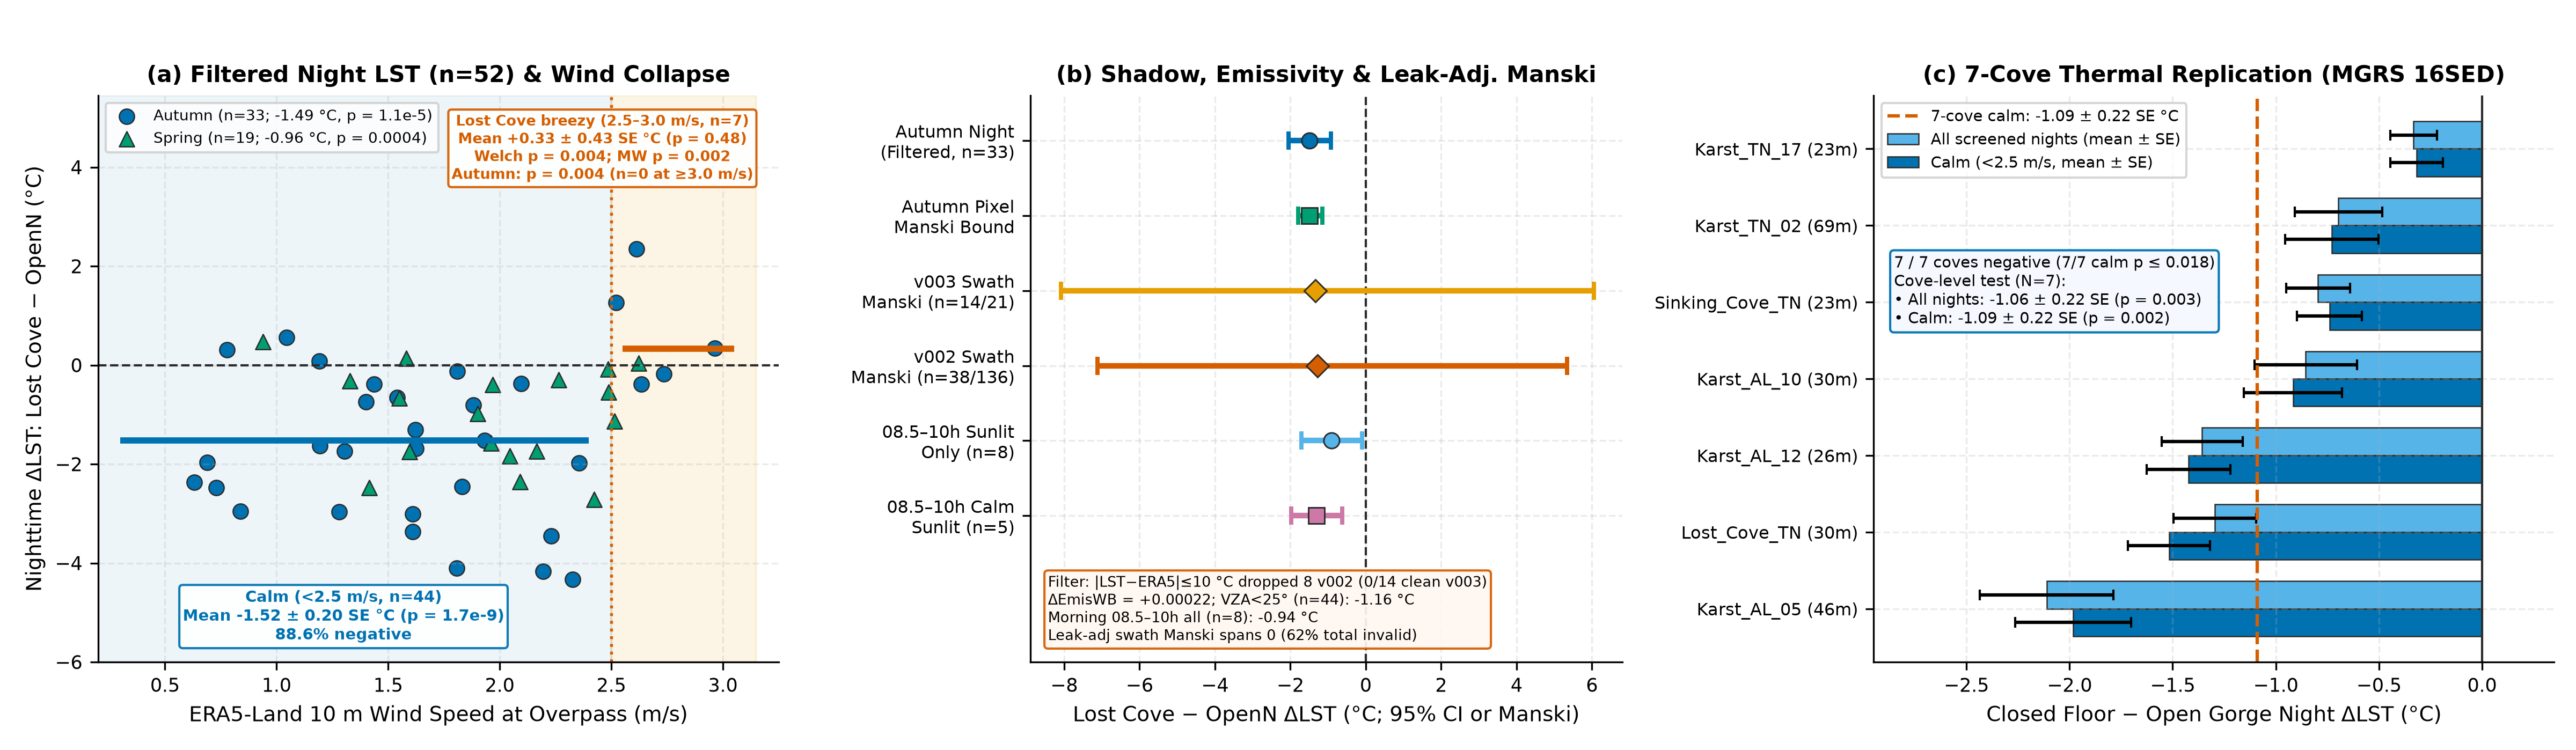
\includegraphics[width=\linewidth]{figures/fig4.png}
\caption{\textbf{Filtered ECOSTRESS confirms nocturnal cooling in spring, autumn, and 7/7 coves.} (a)~Across 52 filtered nights ($|\text{LST}-\text{ERA5}_{t2m}| \le 10^\circ$C), Lost Cove cools in autumn ($-1.49^\circ$C) and spring ($-0.96^\circ$C) under calm winds ($<2.5$~m/s, $-1.52^\circ$C) but collapses over 2.5--3.0~m/s ($+0.33^\circ$C, Welch $p=0.004$). (b)~Controls show negligible emissivity bias ($+0.00022$), calm sunlit morning cooling ($-1.30^\circ$C), negative pixel bounds, and leak-adjusted \texttt{v002}/\texttt{v003} swath Manski bounds spanning zero. (c)~All 7/7 closed basins in tile \texttt{16SED} run colder than open gorges ($-1.09 \pm 0.22^\circ$C SE calm).}
\label{fig:ecostress_thermal}
\end{figure}

Removing the eight corrupted \texttt{ECOv002} scenes clarifies seasonal cooling in Lost Cove relative to elevation-matched Open North Coves. Whereas the unfiltered spring parametric test was distorted by four cloud-leaked passes ($n=23$, mean $-0.37^\circ$C, $p=0.42$), filtered spring nights (February--April, $n=19$) average $-0.96 \pm 0.22^\circ$C (SE, median $-0.67^\circ$C, 84.2\% negative, $t$-test $p=0.00042$, Wilcoxon $p=0.00034$; calm spring $n=17$: $-1.01 \pm 0.24^\circ$C SE, $p=0.00072$). Autumn nights (September--November, $n=33$) average $-1.49 \pm 0.29^\circ$C (SE, median $-1.63^\circ$C, $t$-test $p=1.1 \times 10^{-5}$, Wilcoxon $p=1.0 \times 10^{-5}$; October $n=7$: $-2.07 \pm 0.65^\circ$C SE, $p=0.019$). Across all 52 filtered nights, Lost Cove averages $-1.30 \pm 0.20^\circ$C (SE, $p=3.8 \times 10^{-8}$).

Boundary-layer cold pools should erode once wind mixes the valley atmosphere \citep{whiteman1982}. At Lost Cove, calm nights ($u_{10}<2.5$~m/s, $n=44$) average $-1.52 \pm 0.20^\circ$C (SE, $p=1.7 \times 10^{-9}$, 88.6\% negative), whereas breezy nights ($2.5 \le u_{10} < 3.0$~m/s, $n=7$) shift to $+0.33 \pm 0.43^\circ$C (SE, $p=0.48$; Welch $p=0.0041$, Mann-Whitney $p=0.0019$; season-controlled OLS $\beta=+1.90 \pm 0.52^\circ$C SE, $p=0.00065$; \cref{fig:ecostress_thermal}a). Within autumn alone, calm nights ($n=27, -1.84 \pm 0.27^\circ$C SE) separate cleanly from breezy nights ($n=5, +0.68 \pm 0.51^\circ$C SE; Welch $p=0.0038$, Mann-Whitney $p=0.0015$). Two scope limits apply: zero clean scenes occur at $u_{10} \ge 3.0$~m/s (continuous linear slope across $0.5$--$3.0$~m/s is $r=0.11, p=0.46$, consistent with a regime threshold rather than a linear trend), and wind collapse does not replicate across the six other \texttt{16SED} coves when using Sewanee's point ERA5 wind (paired calm vs.\ breezy $p=0.77$), likely reflecting spatial wind decorrelation 30--90~km south of Sewanee and deeper basin shelter.

Within MGRS tile \texttt{16SED} (single-tile spatial scope), restricting multi-cove analysis to \texttt{v002} granules verified clear over Sewanee ($|\text{LST}-\text{ERA5}_{t2m}| \le 10^\circ$C, excluding 10 Sewanee-flagged leak granules and 16 cloudy-at-Sewanee passes) shows that all 7/7 closed karst basins replicate calm-night cooling individually on both parametric and Wilcoxon tests (\cref{fig:ecostress_thermal}c): \texttt{Lost\_\allowbreak Cove\_TN} ($n=44, -1.52 \pm 0.20^\circ$C SE, $t$ $p=1.7 \times 10^{-9}$, Wilc.\ $p=1.2 \times 10^{-7}$), \texttt{Karst\_\allowbreak AL\_05} ($n=30, -1.98 \pm 0.28^\circ$C SE, $t$ $p=9.4 \times 10^{-8}$, Wilc.\ $p=6.9 \times 10^{-7}$), \texttt{Karst\_\allowbreak AL\_12} ($n=22, -1.42 \pm 0.20^\circ$C SE, $t$ $p=6.0 \times 10^{-7}$, Wilc.\ $p=4.8 \times 10^{-6}$), \texttt{Karst\_\allowbreak AL\_10} ($n=30, -0.92 \pm 0.24^\circ$C SE, $t$ $p=0.00059$, Wilc.\ $p=0.00035$), \texttt{Sinking\_\allowbreak Cove\_TN} ($n=32, -0.74 \pm 0.16^\circ$C SE, $t$ $p=5.3 \times 10^{-5}$, Wilc.\ $p=9.7 \times 10^{-5}$), \texttt{Karst\_\allowbreak TN\_02} ($n=34, -0.73 \pm 0.23^\circ$C SE, $t$ $p=0.0030$, Wilc.\ $p=5.8 \times 10^{-7}$), and \texttt{Karst\_\allowbreak TN\_17} ($n=33, -0.32 \pm 0.13^\circ$C SE, $t$ $p=0.018$, Wilc.\ $p=0.019$), yielding a cove-level calm mean of $-1.09 \pm 0.22^\circ$C (SE, $N=7, p=0.0024$; all screened nights $-1.06 \pm 0.22^\circ$C SE, $p=0.0029$). Artifact checks show negligible emissivity differences ($\Delta\text{EmisWB}=+0.00022$, $<0.02^\circ$C bias), consistent cooling at low view angles ($\text{VZA}<25^\circ, n=44: -1.16 \pm 0.20^\circ$C SE, $p=9.1 \times 10^{-7}$), and persistent calm sunlit morning cooling at 08:30--10:00 solar time ($n=5, -1.30 \pm 0.35^\circ$C SE, $p=0.020$; all $n=8$ morning passes $-0.94 \pm 0.41^\circ$C SE, $p=0.055$, despite $+5.2\%$ higher ray-traced direct morning insolation in Lost Cove; \cref{fig:ecostress_thermal}b).

Despite consistent clear-sky cooling, thermal remote sensing carries an important censoring bound. Clean-scene pixel \citet{manski1990} bounds stay strictly negative ($[-1.79, -1.15]^\circ$C in autumn; $[-1.50, -1.08]^\circ$C overall). At the swath level, properly treating all unflagged cloud-leaked passes ($|\text{LST}-\text{ERA5}_{t2m}| > 10^\circ$C: 9 in \texttt{v002} and 3 non-clean passes in \texttt{v003}) as unobserved yields worst-case bounds spanning zero in both \texttt{v002} ($n=38/136$ clean, 29.8\% leak-adjusted vs.\ 24.1\% raw cloud-flagged, $[-7.12, +5.34]^\circ$C) and \texttt{v003} ($n=14/21$ clean, 23.8\% leak-adjusted vs.\ 10.9\% raw cloud-flagged, $[-8.09, +6.05]^\circ$C), as well as across all 157 combined passes (29.0\% leak-adjusted cloud missingness $[-8.12, +6.28]^\circ$C; total invalid fraction 62.0\% vs.\ 63.3\%, $[-15.93, +14.95]^\circ$C). Although differential missingness between Lost Cove and Open North Coves is small ($<1.3\%$), closing the worst-case fog bound requires ground temperature loggers.

\subsection{25-Year Landsat Persistence, Sensor Limits, and Falsification of P4}
Across 25 years of Roy-harmonized Landsat 5--9 (2000--2024), Lost Cove greens up later than Open North Coves in 88\% of springs (median $+2.45$~d) and senesces earlier in 80\% of autumns (median $-2.53$~d; \cref{fig:landsat_25yr}a). Two sparse-observation outlier years (2007 EOS $+23.6$~d; 2013 SOS $-30.8$~d) widen variance so that unscreened 25-year OLS means are not statistically significant ($\Delta\text{SOS}=+1.62 \pm 1.42$~d SE, $p=0.27$; $\Delta\text{EOS}=-2.22 \pm 1.34$~d SE, $p=0.11$; net $\Delta\text{GSL}=-3.83$~d, or $-5.98$~d excluding 2007 and 2013). Cross-sensor validation against \texttt{HLS v2.0} over 2018--2024 reveals an asymmetric precision limit: 16-day Landsat reproduces interannual autumn $\Delta\text{EOS}$ closely ($r=0.961, p=0.00056$), but fails to track interannual spring $\Delta\text{SOS}$ ($r=-0.041, p=0.93$).

\begin{figure}[t]
\centering
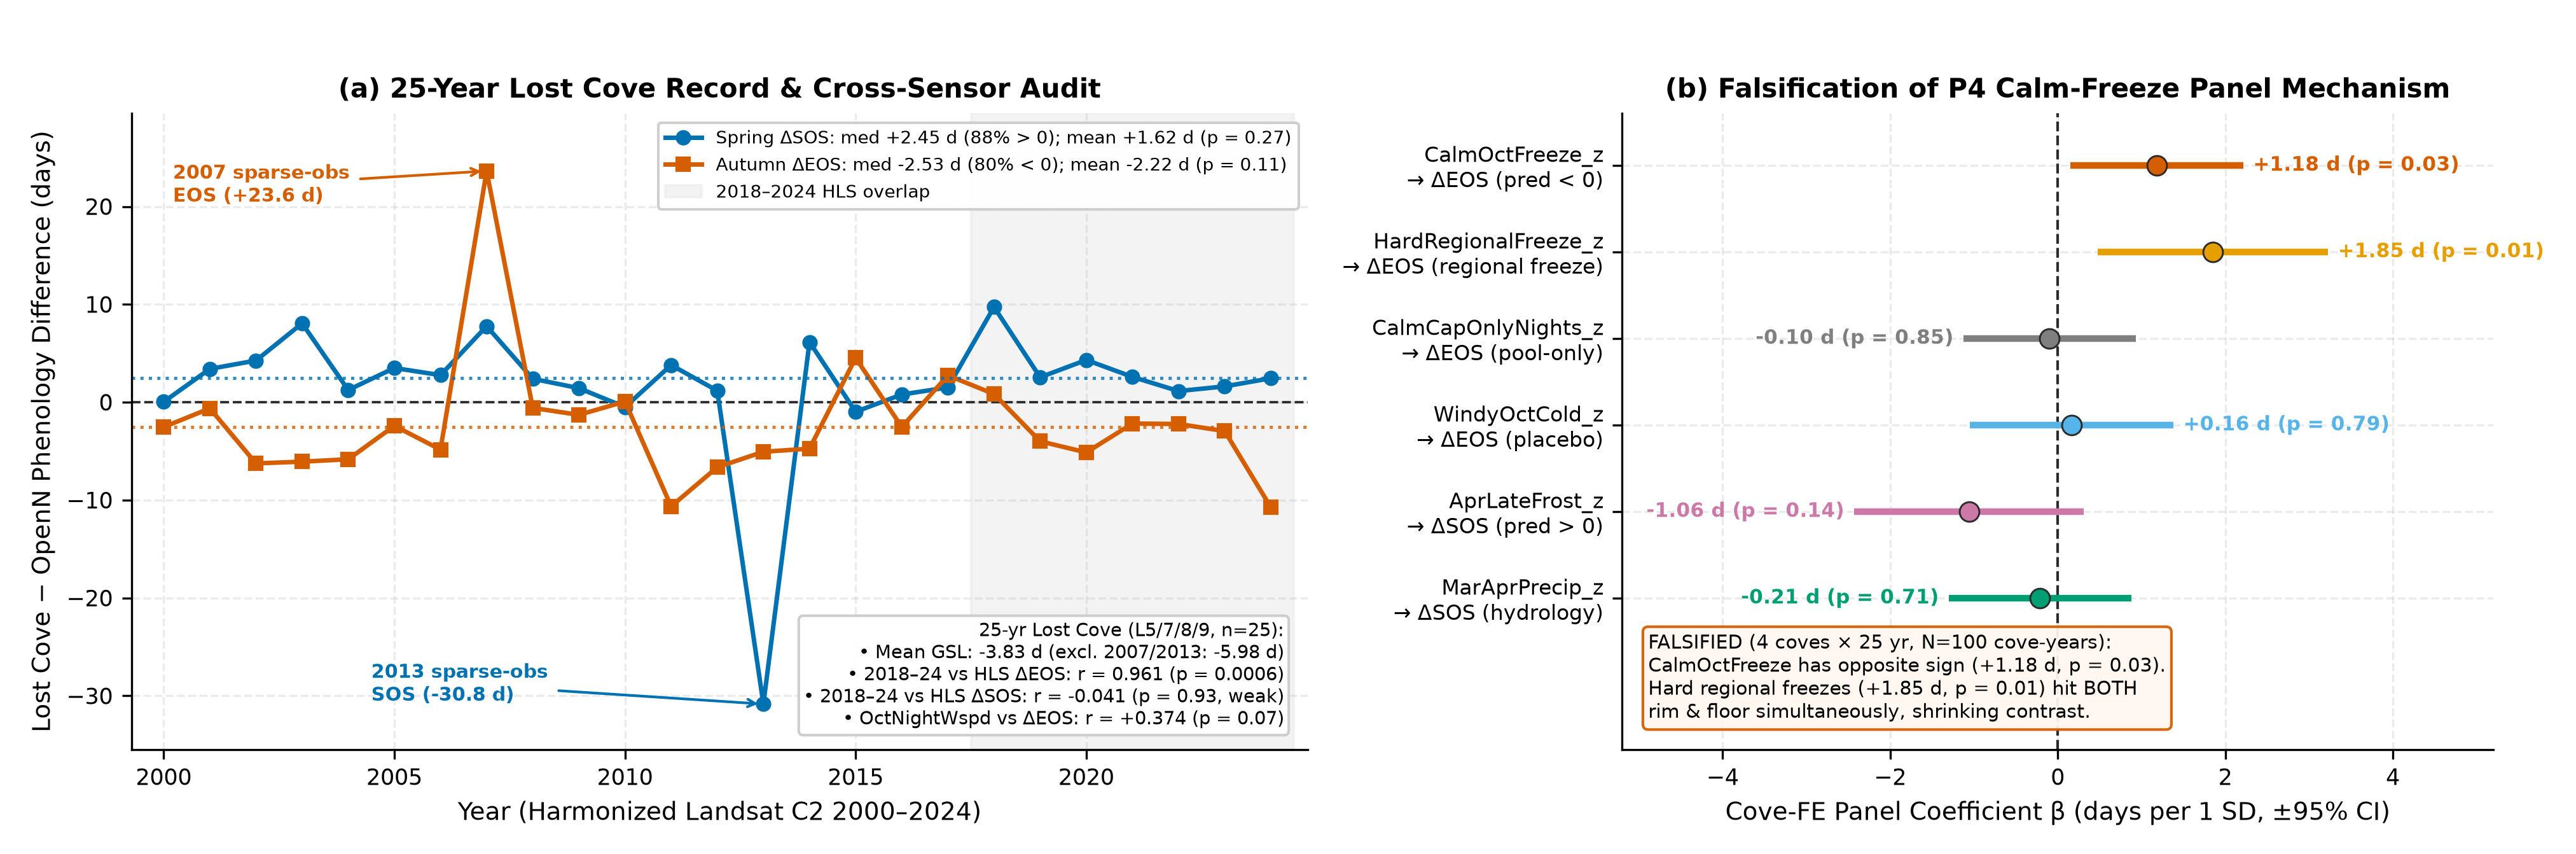
\includegraphics[width=\linewidth]{figures/fig5.png}
\caption{\textbf{25-year Landsat persistence, spring cross-sensor limits, and falsification of P4.} (a)~Harmonized Landsat (2000--2024) records positive spring $\Delta\text{SOS}$ in 88\% of years (median $+2.45$~d, OLS mean $p=0.27$) and negative autumn $\Delta\text{EOS}$ in 80\% (median $-2.53$~d, OLS mean $p=0.11$); over 2018--2024 it tracks \texttt{HLS v2.0} in autumn ($r=0.961, p=0.0006$) but not spring ($r=-0.041, p=0.93$). (b)~Four-cove $\times$ 25-year panel coefficients ($\pm 95\%$ CI): \texttt{CalmOctFreeze} flips positive ($+1.18$~d, $p=0.035$) because hard regional freezes ($+1.85$~d) affect rims and floors together.}
\label{fig:landsat_25yr}
\end{figure}

Our internal four-cove $\times$ 25-year fixed-effects panel test (P4, $N=100$ cove-years) predicted that more calm October freeze nights would make floor-minus-rim $\Delta\text{EOS}$ more negative. The data falsified this prediction with the opposite sign ($\beta=+1.18 \pm 0.53$~d/SD SE, $p=0.035$; \cref{fig:landsat_25yr}b). Decomposing October nights shows that hard regional freezes ($\beta=+1.85 \pm 0.70$~d/SD SE, $p=0.014$) push both upper rims and basin floors below freezing together, compressing the floor--rim contrast, while marginal pool-only nights ($\beta=-0.10 \pm 0.52$~d/SD SE, $p=0.85$) and windy cold placebos ($\beta=+0.16 \pm 0.62$~d/SD SE, $p=0.79$) are indistinguishable from zero. Likewise, nighttime October wind speed (\texttt{OctNightWspd}) is non-significant in Lost Cove ($r=0.37, p=0.065$; daily wind $r=0.44, p=0.027$ is unconfirmed in the 4-cove panel). At 16-day Landsat revisit precision, closed-karst compression therefore appears as a chronic structural microclimate effect rather than a single-storm interannual toggle.
